% 2007 年福建卷文科第 6 题：正方体 ABCD-A1B1C1D1，E、F、G、H 分别为
%   AA1、AB、BB1、B1C1 的中点，图中画出异面直线 EF 与 GH。
% 来源 PDF：gaokaomath-src/普通高考/2007/2007福建文.pdf
% SHA-256：96ffeae7fae0016108ed33e565abdf5983e06aef19f6452a8b4c8c5e5e4e58d0
% 原页：2007福建文.pdf 第 1 页（A3 三栏）第 1 栏，书页码 369。
% 重绘依据：按原页斜投影（前表面 ABB1A1、右表面 BCC1B1、上表面 A1B1C1D1）
%   与 A-D、D-C、D-D1 三条虚线重绘，E、F、G、H 均取棱的中点。
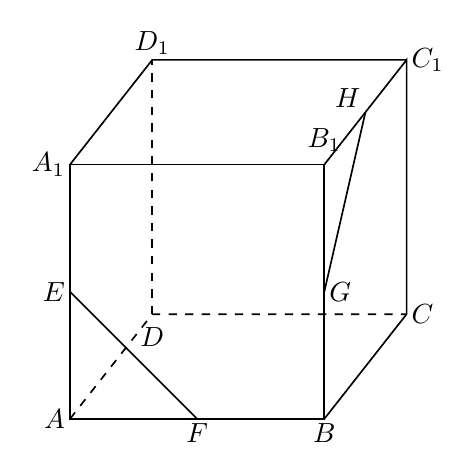
\begin{tikzpicture}[scale=0.95, semithick,
  every node/.style={inner sep=1.5pt}]

  \coordinate (A)  at (0.0,0.0);
  \coordinate (B)  at (3.4,0.0);
  \coordinate (C)  at (4.5,1.4);
  \coordinate (D)  at (1.1,1.4);
  \coordinate (A1) at (0.0,3.4);
  \coordinate (B1) at (3.4,3.4);
  \coordinate (C1) at (4.5,4.8);
  \coordinate (D1) at (1.1,4.8);
  \coordinate (E)  at (0.0,1.7);
  \coordinate (F)  at (1.7,0.0);
  \coordinate (G)  at (3.4,1.7);
  \coordinate (H)  at (3.95,4.1);

  % 可见的棱
  \draw (A) -- (B) -- (B1) -- (A1) -- cycle;
  \draw (B) -- (C) -- (C1) -- (B1);
  \draw (A1) -- (D1) -- (C1);

  % 被遮挡的棱
  \draw[dashed] (A) -- (D) -- (C);
  \draw[dashed] (D) -- (D1);

  % 异面直线 EF 与 GH
  \draw (E) -- (F);
  \draw (G) -- (H);

  \node[left] at (A) {$A$};
  \node[below] at (B) {$B$};
  \node[right] at (C) {$C$};
  \node[below=3pt] at (D) {$D$};
  \node[left] at (A1) {$A_1$};
  \node[above=3pt] at (B1) {$B_1$};
  \node[right] at (C1) {$C_1$};
  \node[above] at (D1) {$D_1$};
  \node[left] at (E) {$E$};
  \node[below] at (F) {$F$};
  \node[right] at (G) {$G$};
  \node[above left] at (H) {$H$};
\end{tikzpicture}
